\documentclass{article}
\usepackage[utf8]{inputenc}
\usepackage{graphicx}
\usepackage{parskip}
\usepackage{xcolor}
\usepackage{textcomp}
\usepackage{hyperref}
\hypersetup{
    colorlinks=true,
    linkcolor=blue,
    filecolor=magenta,      
    urlcolor=cyan,
}
\usepackage{listings}
\lstset{language=C,
                backgroundcolor = \color{lightgray},
                showstringspaces = false,
                basicstyle=\ttfamily,
                keywordstyle=\color{blue}\ttfamily,
                stringstyle=\color{red}\ttfamily,
                commentstyle=\color{green}\ttfamily,
                morecomment=[l][\color{magenta}]{\#}
}

\title{Breakout - Code Documentation}
\author{By \\ Umang Deshpande and Akshay Hegde}
\date{June 2017}

\begin{document}
\maketitle

\section{Program Code}
\qquad The git repository for the complete code can be found \href{https://github.com/eYSIP-2017/eYSIP-2017_Game_Development-TI-RTOS/tree/master/Breakout_Final}{here}. It contains the complete project folder used in CCS. 
\begin{itemize}
  \item The console support libraries(including the font libraries) are present in the \href{https://github.com/eYSIP-2017/eYSIP-2017_Game_Development-TI-RTOS/tree/master/Breakout_Final/Console}{Console} folder. 
  \item The game objects are present in the \href{https://github.com/eYSIP-2017/eYSIP-2017_Game_Development-TI-RTOS/tree/master/Breakout_Final/Objects}{Objects} folder.
    \item The game screens are present in the \href{https://github.com/eYSIP-2017/eYSIP-2017_Game_Development-TI-RTOS/tree/master/Breakout_Final/Screens}{Screens} folder.
  \item game.c is the main file. This contains the two basic tasks part of RTOS, with their internal state machines. Additional functions are used from above libraries.
\end{itemize}

\section{Main Code}
\qquad Firstly, following headers are included:
  \begin{lstlisting}[basicstyle = \small, language = C]
/* XDC module Headers */
#include <xdc/std.h>
#include <xdc/runtime/System.h>

#include <xdc/runtime/Log.h>                
//needed for any Log_info() call
#include <xdc/cfg/global.h>                 
//header file for statically defined objects/handles
#include <xdc/runtime/Log.h>                
//needed for any Log_info() call


/* BIOS module Headers */
#include <ti/sysbios/BIOS.h>
#include <ti/sysbios/knl/Clock.h>
#include <ti/sysbios/knl/Task.h>
#include <ti/sysbios/knl/Semaphore.h>

/* Standard C Libraries */
#include <stdint.h>
#include <stdlib.h>
#include <stdbool.h>

/* Include header files for ADC,Timer 
and Interrupt functions */
#include "inc/hw_types.h"
#include "inc/hw_memmap.h"
#include "driverlib/gpio.h"
#include "inc/tm4c123gh6pm.h"
#include "driverlib/debug.h"
#include "driverlib/pin_map.h"
#include "driverlib/adc.h"
#include "driverlib/interrupt.h"
#include "driverlib/timer.h"
#include <time.h>

// ROM Functions Header
#define TARGET_IS_BLIZZARD_RB1
#include "driverlib/rom.h"

// Custom Console Header Functions
#include "Console/consoleInit.h"
#include "Console/glcd.h"
#include "Console/gameDisplay.h"
#include "Console/tones.h"
#include "Objects/gameObjects.h"
#include "Screens/gameScreens.h"
  \end{lstlisting}
\begin{itemize}
  \item XDC Headers handle XDCTools as part of RTOS, which aid in debugging.
  \item BIOS module headers allow use of Tasks and Semaphore definitions.
  \item \texttt{stdint.h} Headers allow use of \texttt{uint32} variables, stdbool allows use of \texttt{stdbool.h} variables, \texttt{stdlib.h} allows randomization function \texttt{rand()} to be called.
  \item For the timer,timer interrupt and ADC functions used in \texttt{Timer2\_ISR}(Task Scheduler) and in ADC Input code, the different libraries for Tiva C are included
  \item \texttt{rom.h} Allows the use of ROM functions for the given board.
  \item \begin{itemize}
    \item The Console headers provide developer level functions to the console, so that initialization can be performed using a single function \texttt{\_init\_()}.
    \item GLCD functions for basic GLCD refresh, sending commands and sending data are obtained from \texttt{glcd.h} header.
    \item Various game objects(Like a graphic of a particular dimension) can be displayed on screen using certain specific functions in \texttt{gameDisplay.h}.
    \item Different beeps and music can be played through the functions defined in \texttt{tones.h}.
    \item The different game objects are designed and their hex arrays are stored in \texttt{gameObjects.h}.
    \item The game screens are designed using Paint, converted to Hex from BMP format, and then preloaded in the form of hex arrays in \texttt{gameScreens.h}.
  \end{itemize}
\end{itemize}
\qquad Following this, define all global variables are defined as follows:
  \begin{lstlisting}[basicstyle = \small, language = C]

/* Global Variables
 */

uint32_t ui32ADC0Value,latency, tickCount; 
uint32_t specialTimeCount, pinName, baseName;
uint8_t ui8XAxisAvg, ui8XAxisPrev = 64;
signed char hit[64];
signed int paddleXPos, paddleXPrev;
unsigned char victoryCheck, ballXPos,ballYPos;
unsigned char ballXPrev, ballYPrev;
unsigned int ballXMapInt, scoreInt, lifeCount = 3;
unsigned int ballMovSpeed = 325, paddleSpeed = 2;
unsigned int lifeCountTemp;
char score_str[4];
  \end{lstlisting}
\begin{itemize}
  \item \texttt{ui32ADC0Value} is used for ADC Input Buffer.
  \item \texttt{latency} defines game screen refresh latency.
  \item \texttt{tickCount} is used for Task Scheduling in \texttt{Timer\_ISR}.
  \item \texttt{specialTimeCount} is used to count 10 seconds in the SPECIAL mode of the paddle in \texttt{Timer1\_ISR}.
  \item \texttt{pinName},\texttt{baseName} and \texttt{flag} are used for Switch selection. \texttt{baseName} is the port to which the switch belongs to. \texttt{pinName} is the actual pin to which the switch is connected.
  \item \texttt{ui8XAxisAvg} is used to read ADC value. And \texttt{ui8XAxisPrev} holds the previous sampled value of the ADC, for clearing purposes.
  \item \texttt{hit[64]} holds the value of the hit for each block that can be displayed on screen.
  \item \texttt{paddleXPos} is used to hold the sticky position of the paddle with response to the Thumbstick ADC. The previous paddle position is stored in \texttt{paddleXPrev}.
  \item \texttt{victoryCheck} flag is used to check for victory condition(whether all blocks are cleared).
  \item \texttt{ballXPos, ballYPos, ballXPrev} and \texttt{ballYPrev} is used to monitor the present and previous positions of the ball.
  \item \texttt{ballXMapInt} is used to map ball position to corresponding block position.
  \item \texttt{scoreInt} is used to monitor score where \textt{score\_str[4]} stores the score in string format to be displayed on GLCD.
  \item \texttt{lifeCount} is the total number of lives available to the player at the start of game, where \texttt{lifeCountTemp} is the live monitoring of pending lives during gameplay.
  \item \texttt{ballMovSpeed} controls the delay between subsequent ball display. Smaller the value, faster is the ball.
  \item \texttt{paddleSpeed} is used to control the speed of the paddle. Larger the value, greater the speed.
\end{itemize}
\qquad All the different states for the various state machines used are enlisted as follows:
  \begin{lstlisting}[basicstyle = \small, language = C]
/*
 * Enumeration of States for State Machines
 */
enum modes
{
    // Different game states(Classified 
    // because of different I/O behaviour in each state)
    MENU,
    INSTRUCTIONS,
    SETTINGS,
    GAMEPLAY,
    VICTORY,
    GAMEOVER
};
// Initialization
enum modes mode = MENU;
  \end{lstlisting}
  \texttt{mode} enumerated variable is thus initially in \texttt{MENU} state.
    \begin{lstlisting}[basicstyle = \small, language = C]
enum menuModes menuMode = ENTRY;
// Different Paddle States(Different paddle sizes 
// upon hit of BLOCK_MAGIC2)
enum gameplayChanges
{
    NORMAL,
    SPECIAL
};
// Initialization
enum gameplayChanges gameplayChange;
  \end{lstlisting}
\texttt{gameplayChange} enumerated variable is thus initialized.
\begin{lstlisting}[basicstyle = \small, language = C]
// Different Gameplay Internal States
// (Different I/O behaviour in different states)
enum gameplayModes
{
    ENTER,
    DEATH,
    REENTER,
    ALWAYS
};
// Initialization
enum gameplayModes gameplayMode = ENTER;
  \end{lstlisting}
    \texttt{gameplayMode} enumerated variable is thus initialized to \texttt{ENTER}.
\begin{lstlisting}[basicstyle = \small, language = C]
// Different Menu Internal States
// (Certain functions are called upon 
// entry, rest are performed throughout)
enum menuModes
{
    ENTRY,
    THROUGHOUT
};
// Initialization
enum menuModes menuMode = ENTRY;
  \end{lstlisting}
    \texttt{menuMode} enumerated variable is thus initialized to \texttt{ENTRY}.
\begin{lstlisting}[basicstyle = \small, language = C]
// Cursor States
enum cursorPositions
{
    ONE,
    TWO,
    THREE
};
// Initialization
enum cursorPositions cursorPos;
  \end{lstlisting}
    \texttt{cursorPos} enumerated variable is thus initialized.
        \begin{lstlisting}[basicstyle = \small, language = C]
// Enumeration of Difficulties
// (Different brick composition and 
// number of lives on game start)
enum difficulties
{
    EASY, // More Easy Bricks, 3 Lives
    MEDIUM, // More Medium Bricks, 2 Lives
    HARD // More Hard Bricks, 1 Lifes
};
// Initialization
enum difficulties difficulty;
  \end{lstlisting}
    \texttt{difficulty} enumerated variable is thus initialized.
\begin{lstlisting}[basicstyle = \small, language = C]
// Enumeration of different ballspeed states
enum ballSpeeds
{
    SLOW,
    FAST,
    FASTER
};
// Initialization
enum ballSpeeds ballSpeed = FAST;
  \end{lstlisting}
\texttt{ballSpeed} enumerated variable is thus initialized to \texttt{FAST}.
\begin{lstlisting}[basicstyle = \small, language = C]
// Different Ball States(Directions)
enum directions
{
    INIT, 
    // For Initial Ball Position 
    // at centre on gameplay entry/ re entry
    UP_LEFT,
    UP_RIGHT,
    DOWN_RIGHT,
    DOWN_LEFT,
};
// Initialization
enum directions direction = INIT;
  \end{lstlisting}
\texttt{direction} enumerated variable is thus initialized to \texttt{INIT}.
\begin{lstlisting}[basicstyle = \small, language = C]
// Different Block Type(States for Blocks)
enum blocks
{
    NONE, // No Block
    BLOCK_HARD, // Takes 3 hits to disappear
    BLOCK_MED, // Takes 2 hits to disappear
    BLOCK_EASY, // Takes 1 hit to disappear
    BLOCK_MAGIC1, 
    // Delivers 1 hit to all surrounding blocks 
    // and itself disappears
    BLOCK_MAGIC2 // Increases Paddle Size for 10 Seconds
};
// Initialization of blocks(Maximum 
// of 64 blocks can be accomodated on screen)
enum blocks block[64];
  \end{lstlisting}
    \texttt{block} enumerated variable is thus initialized. \\ \\
\qquad Following this, various functions are defined as follows: \\ \\
\texttt{ballMovement()}:\\ This function has the ball direction state machine, which continuously controls ball motion. Ball is reflected off the left,right, top walls and also off the paddle. It also checks for brick collision at all times, and is reflected off of the brick if it is present and also delivers 1 hit to the brick. Initially, it also checks whether all bricks are cleared(for victory condition).
The state machine implemented here is as follows:
\begin{center}
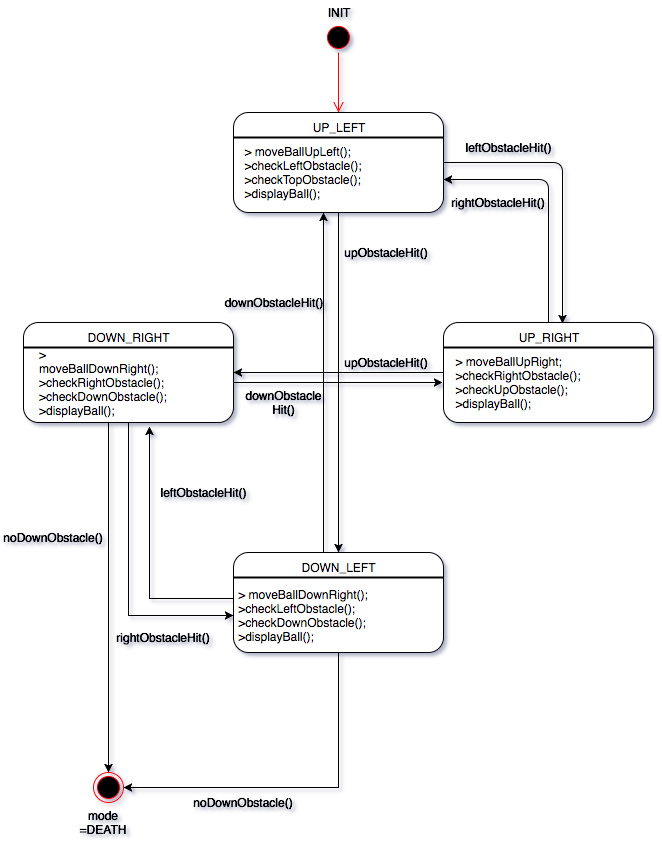
\includegraphics[width=9cm, height=12cm]{ballDirectionStatemachine}
\\ {\small Fig a: Ball Direction State Machine}
\end{center}
\qquad The actual function performs additional checks, and the obstacle hits are inbuilt into certain if else cases within the switch case. The \texttt{blockclear()} function implements the block type state machine as follows:
\begin{center}
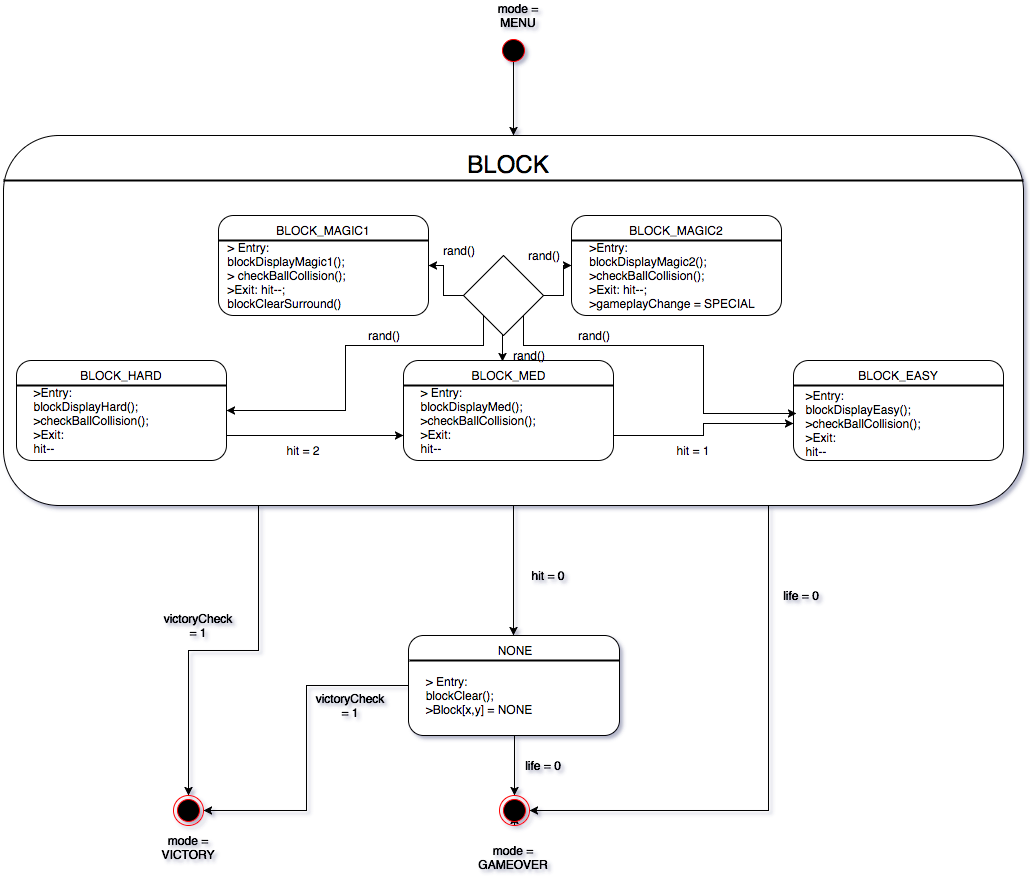
\includegraphics[width=12cm, height=10cm]{brickTypeStatemachine}
\\ {\small Fig b: Block Type State Machine}
\end{center}
The \texttt{blockclear()} function(Fully documented) is available in the \texttt{gameDisplay.h}.
\newpage
\begin{lstlisting}[basicstyle = \small, language = C]
void ballMovement(void)
{
    // Victory condition check
    volatile unsigned char arrayCount = 0;
    victoryCheck = 1;
    for(arrayCount = 0; arrayCount < 32; arrayCount++)
    {
        // If Brick is detected then break off the check
        if(block[arrayCount] != NONE)
        {
            victoryCheck = 0;
            break;
        }
    }
    switch(direction){
    case INIT:
        // Initially ball is display at the centre of 
        // 7th BallXPos and 7th Page
        ballDisplay(ballInit);
        // Set direction as UP_LEFT
        direction = UP_LEFT;
        break;
    case UP_LEFT:
        // Change ball Coordinates
        if(ballXPos > 0)
            ballXPos--;
        if (ballYPos > 0)
            ballYPos--;

        // Maps ball position to correspond to brick 
        // position, there are 16 Ball X Positions
        // and 8 Brick Positions, hence divided by 2.
        ballXMapInt = (ballXPos/2);

        // Check whether there is a brick to the left, 
        // if so, delivers 1 hit and is reflected UP_RIGHT
        if(block[ballXMapInt + (8*(ballYPos+1))] != NONE)
        {
            blockClear(ballXMapInt, (ballYPos+1));
            direction = UP_RIGHT;
            // Do not display the ball, roll back 
            // UP_LEFT ball co ordinates changes
            ballXPos++;
            ballYPos++;
            // Break out of the switch case
            break;
        }
        // Check whether there is a brick to the top, if so, 
        // delivers 1 hit and is reflected DOWN_LEFT
        else if(block[ballXMapInt + (8*ballYPos)] != NONE)
        {
            blockClear(ballXMapInt, ballYPos);
            direction = DOWN_LEFT;
            // Roll Back Ball co-ordinates change
            ballXPos++;
            ballYPos++;
            break;
        }
        // No Brick Detected
        else
        {
            /* Display the ball as per UP_LEFT coordinates 
            change(Since ball is 4x4, and we can move in 
            8x8 frames using GLCD. There are two ball displays 
            in different quadrants for fluider ball motion)
            */
            ballDisplay(ball3);
            millis(ballMovSpeed/2);
            ballDisplay(ball1);
            millis(ballMovSpeed/2);
            // Check for left wall collision
            if(ballXPos == 0)
            {
                direction = UP_RIGHT;
                // Check for top left corner collision
                if(ballYPos == 0)
                {
                    direction = DOWN_RIGHT;
                    break;
                }
                break;
            }
            // Check for top wall collision
            if(ballYPos == 0)
                direction = DOWN_LEFT;
            break;
        }
    case UP_RIGHT:
        // Change ball Coordinates
        if(ballXPos < 15)
            ballXPos++;
        if (ballYPos > 0)
            ballYPos--;

        // Maps ball position to correspond to brick 
        // position, there are 16 Ball X Positions
        // and 8 Brick Positions, hence divided by 2.
        ballXMapInt = (ballXPos/2);

        // Check whether there is a brick to the right, 
        // if so, delivers 1 hit and is reflected UP_LEFT
        if(block[ballXMapInt + (8*(ballYPos+1))] != NONE)
        {
            blockClear(ballXMapInt, (ballYPos+1));
            direction = UP_LEFT;
            // Roll Back Ball co-ordinates change
            ballXPos--;
            ballYPos++;
            break;
        }
        // Check whether there is a brick to the top, if so, 
        // delivers 1 hit and is reflected DOWN_RIGHT
        else if(block[ballXMapInt + (8*ballYPos)] != NONE)
        {
            blockClear(ballXMapInt, ballYPos);
            direction = DOWN_RIGHT;
            // Roll Back Ball co-ordinates change
            ballXPos--;
            ballYPos++;
            break;
        }
        // No Brick Detected
        else
        {
            /* Display the ball as per UP_RIGHT co ordinates 
            change(Since ball is 4x4, and we can move in 
            8x8 frames using GLCD, there are two ball displays 
            in different quadrants for fluider ball motion) */
            ballDisplay(ball3);
            millis(ballMovSpeed/2);
            ballDisplay(ball0);
            millis(ballMovSpeed/2);
            // Check for right wall collision
            if(ballXPos == 15)
            {
                direction = UP_LEFT;
                // Check for top right corner collision
                if(ballYPos == 0)
                {
                    direction = DOWN_LEFT;
                    break;
                }
            }
            // Check for top wall collision
            if(ballYPos == 0)
                direction = DOWN_RIGHT;
            break;
        }
    case DOWN_RIGHT:
        // Change ball co-ordinates
        if(ballXPos < 15)
            ballXPos++;
        if (ballYPos < 7)
            ballYPos++;

        /* Maps ball position to correspond to brick position,
        there are 16 Ball X Positions and 8 Brick Positions, 
        hence divided by 2. */
        ballXMapInt = (ballXPos/2);
        // Check whether there is a brick to the right,
        // if so, delivers 1 hit and is reflected DOWN_LEFT
        if(block[ballXMapInt + (8*(ballYPos-1))] != NONE)
        {
            blockClear(ballXMapInt, (ballYPos-1));
            direction = DOWN_LEFT;
            // Roll Back Ball co-ordinates change
            ballXPos--;
            ballYPos--;
            break;
        }
        // Check whether there is a brick down, if so,
        // delivers 1 hit and is reflected UP_RIGHT
        else if(block[ballXMapInt + (8*ballYPos)] != NONE)
        {
            blockClear(ballXMapInt, ballYPos);
            direction = UP_RIGHT;
            // Roll Back Ball co-ordinates change
            ballXPos--;
            ballYPos--;
            break;
        }
        // No Brick Detected
        else
        {
            // Display first ball in the two ball motion
            ballDisplay(ball0);
            millis(ballMovSpeed/2);
            // Check for right wall collision
            if(ballXPos == 15)
            {
                direction = DOWN_LEFT;
            }
            // Check for ball in bottom row
            if(ballYPos == 7)
            {
                // Based on size of paddle, 
                // different checks are performed 
                // for bouncing off 
                // the paddle
                switch(gameplayChange){
                case NORMAL:
                    // Normal sized paddle, 
                    // check whether ball position 
                    // matches paddle position
                    if((ballXPos >= ((paddleXPos-6)/8)) 
                    && (ballXPos <= ((paddleXPos + 6)/8)))
                    {
                        // If paddle is present, is 
                        // reflected off
                        direction = UP_RIGHT;
                        paddleBeep();
                        break;
                    }
                    else
                    {
                        // If paddle is not present, 
                        // then a life is lost
                        gameplayMode = DEATH;
                        break;
                    }
                case SPECIAL:
                    // Larger sized paddle, check 
                    // whether ball position matches 
                    //paddle position
                    if((ballXPos >= ((paddleXPos-12)/8)) 
                    && (ballXPos <= ((paddleXPos + 12)/8)))
                    {
                        // If special paddle is present, 
                        // is reflected off
                        direction = UP_RIGHT;
                        paddleBeep();
                        break;
                    }
                    else
                    {
                        // If special paddle is not present, 
                        // then a life is lost
                        gameplayMode = DEATH;
                        break;
                    }
                }
            }
            // If ball is not in the lowest page, then 
            // display second ball position
            ballDisplay(ball3);
            millis(ballMovSpeed/2);
            break;
        }
    case DOWN_LEFT:
        // Change ball co-ordinates
        if(ballXPos > 0)
            ballXPos--;
        if (ballYPos < 7)
            ballYPos++;

        /* Maps ball position to correspond to brick 
        position, there are 16 Ball X Positions
        and 8 Brick Positions, hence divided by 2 */
        ballXMapInt = (ballXPos/2);
        /* Check whether there is a brick to the left, 
        if so, delivers 1 hit and is reflected DOWN_RIGHT
        */
        if(block[ballXMapInt + (8*(ballYPos-1))] != NONE)
        {
            blockClear(ballXMapInt, (ballYPos-1));
            direction = DOWN_RIGHT;
            // Roll Back Ball co-ordinates change
            ballXPos++;
            ballYPos--;
            break;
        }
        // Check whether there is a brick down, 
        // if so, delivers 1 hit and is reflected 
        // UP_LEFT
        else if(block[ballXMapInt + (8*ballYPos)] != NONE)
        {
            blockClear(ballXMapInt, ballYPos);
            direction = UP_LEFT;
            // Roll Back Ball co-ordinates change
            ballXPos++;
            ballYPos--;
            break;
        }
        // No Brick detected
        else
        {
            // Display first ball in the two ball motion
            ballDisplay(ball3);
            millis(ballMovSpeed/2);
            // Check for left wall collision
            if(ballXPos == 0)
            {
                direction = DOWN_RIGHT;
            }
            // Check for ball in bottom row
            if(ballYPos == 7)
            {
                /* Based on size of
                paddle, different checks are 
                performed for bouncing off 
                the paddle */
                switch(gameplayChange){
                case NORMAL:
                    // Normal sized paddle, 
                    // check whether ball
                    // position matches 
                    // paddle position
                    if((ballXPos >= ((paddleXPos-6)/8)) 
                    && (ballXPos <= ((paddleXPos + 6)/8)))
                    {
                        // If paddle is present, is 
                        // reflected off
                        direction = UP_LEFT;
                        paddleBeep();
                        break;
                    }
                    else
                    {
                        // If paddle is not present, 
                        // then a life is lost
                        gameplayMode = DEATH;
                        break;
                    }
                case SPECIAL:
                    // Larger sized paddle, check 
                    // whether ball position matches paddle 
                    // position
                    if((ballXPos >= ((paddleXPos-12)/8)) 
                    && (ballXPos <= ((paddleXPos + 12)/8)))
                    {
                        // If special paddle is present, 
                        // is reflected off
                        direction = UP_LEFT;
                        paddleBeep();
                        break;
                    }
                    else
                    {
                        // If special paddle is not present, 
                        // then a life is lost
                        gameplayMode = DEATH;
                        break;
                    }
                }
            }
            // If ball is not in the lowest page, 
            // then display second ball position
            ballDisplay(ball2);
            millis(ballMovSpeed/2);
            break;

        }
    }
}
  \end{lstlisting}
\texttt{readInput()}: \\ This function switches input behaviour based on the overall state of the game. It includes initial menu navigation using a cursor, which switches between settings, instructions and menu screen using on board switch presses alone. Once in gameplay mode, input is through the ADC Joystick, and Joystick ADC is mapped as per paddle size. Is implemented as a task in RTOS, initialized with readInputSem Semaphore. The overall state machine for the game is given by Fig b. \\
\\ \qquad But the \texttt{readInput()} task handles only the input functions within each state. Output functions are handled by the \texttt{displayOutput()} task. Hence two different instances of the same state machine are called with each task, each with different internal functions. \\
\\ \qquad Additionally, the \texttt{readInput()} task also runs the internal state machine for the cursor position within the \textit{MENU} and \textiy{SETTINGS} state.
\begin{center}
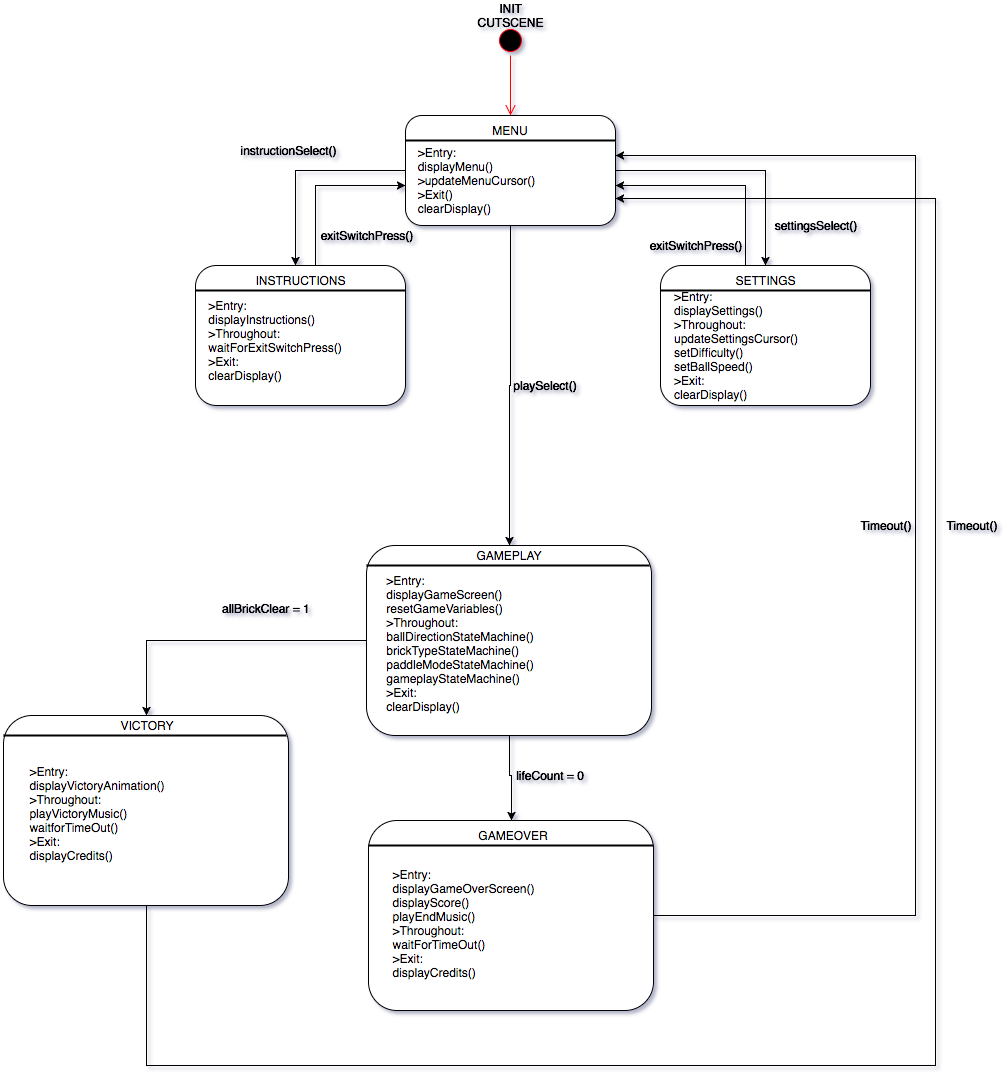
\includegraphics[width=14cm, height=15cm]{gameStateMachine}
\\ {\small Fig c: Game State Machine}
\end{center}
  \begin{lstlisting}[basicstyle = \small, language = C]
void readInput(void)
{
    while(1)
    {

        /*  Semaphore_pend(*sem, wait/timeout) 
         *  decrements the semaphore by 1.
         *  Until semaphore value is zero task 
         *  is blocked.
         *
         */
        Semaphore_pend(readInputSem, BIOS_WAIT_FOREVER);

        // Once Semaphore is posted, Switching State 
        // Machine uses different game states to dictate 
        // input behaviour
        switch(mode){
        // In the MENU screen
        case MENU:
            // Cursor Position States in Menu
            switch(cursorPos){
            case ONE:
                // Pointing to PLAY option
                if(detectKeyPress(1) == 1)
                {
                    // Once RIGHT SWITCH is pressed, 
                    // start gameplay
                    mode = GAMEPLAY;
                    gameplayMode = ENTER;
                    // Beep Feedback
                    entryBeep();
                    glcd_clearDisplay();
                }
                else if(detectKeyPress(2) == 1)
                {
                    // Once DOWN SWITCH is pressed, 
                    // cursor points to INSTRUCTIONS 
                    // option
                    cursorPos = TWO;
                    blockBeep();
                }
                break;
            case TWO:
                // Pointing to INSTRUCTIONS option
                if(detectKeyPress(1) == 1)
                {
                    // Once RIGHT SWITCH is pressed, 
                    // move to INSTRUCTIONS screen
                    mode = INSTRUCTIONS;
                    // Beep feedback
                    entryBeep();
                    glcd_clearDisplay();
                }
                else if(detectKeyPress(0) == 1)
                {
                    // If UP SWITCH is pressed, 
                    // cursor points to PLAY option
                    cursorPos = ONE;
                    blockBeep();
                }
                else if(detectKeyPress(2) == 1)
                {
                    // If DOWN SWITCH is pressed, 
                    // cursor points to SETTINGS option
                    cursorPos = THREE;
                    blockBeep();
                }
                break;
            case THREE:
                // Pointing to SETTINGS option
                if(detectKeyPress(1) == 1)
                {
                    // If RIGHT SWITCH is pressed, 
                    // move to SETTINGS screen
                    mode = SETTINGS;
                    entryBeep();
                    glcd_clearDisplay();
                    glcd_write(settingsScreen);
                    // Cursor position at one in the 
                    // Settings Screen(Pointing to DIFFICULTY 
                    // option)
                    cursorPos = ONE;
                }
                else if(detectKeyPress(0) == 1)
                {
                    // If UP SWITCH is pressed, cursor 
                    // points to INSTRUCTIONS option
                    cursorPos = TWO;
                    blockBeep();
                }
                break;
            }
            break;
            // In the INSTRUCTIONS screen
            case INSTRUCTIONS:
                if(detectKeyPress(3) == 1)
                {
                    // If LEFT SWITCH is pressed, go back 
                    // to MENU screen
                    menuMode = ENTRY;
                    mode = MENU;
                    glcd_clearDisplay();
                }
                break;
            // In the SETTINGS screen
            case SETTINGS:
                // Cursor position states in SETTINGS
                switch(cursorPos){
                case ONE:
                    // Pointing to DIFFICULTY option
                    if(detectKeyPress(1) == 1)
                    {
                        difficulty = HARD; 
                        // If RIGHT SWITCH is pressed, 
                        // difficulty is set to HARD
                        lifeCount = 1; // Only One Life
                    }
                    else if(detectKeyPress(3) == 1)
                    {
                        difficulty = EASY; 
                        // If LEFT SWITCH is pressed,
                        // difficulty is set to EASY
                        lifeCount = 3; // Three Lives
                    }
                    else if(detectKeyPress(4) == 1)
                    {
                        difficulty = MEDIUM; 
                        // If HAT SWITCH is pressed, 
                        // difficulty is set to MEDIUM
                        lifeCount = 2; // Two Lives
                    }
                    else if(detectKeyPress(0) == 1)
                    {
                        // If UP SWITCH is pressed, 
                        // move back to MENU Screen
                        mode = MENU;
                        menuMode = ENTRY;
                    }
                    else if(detectKeyPress(2) == 1)
                        cursorPos = TWO; 
                        // If DOWN SWITCH is pressed, 
                        // cursor points to BALL SPEED
                        // option
                    break;
                case TWO:
                    // Pointing to BALL SPEEDS option
                    if(detectKeyPress(1) == 1)
                    {
                        // If RIGHT SWITCH is pressed, 
                        // then ball speed is set to the 
                        // fastest option. Also correspondingly
                        // paddle movement is set to a 
                        faster speed for a balanced gameplay
                        ballSpeed = FASTER;
                        ballMovSpeed = 175;
                        paddleSpeed = 4;
                    }
                    else if(detectKeyPress(3) == 1)
                    {
                        // If LEFT SWITCH is pressed, 
                        // then ball speed is set to the 
                        // slowest option. Also correspondingly
                        // paddle movement is set to a slower 
                        // speed for a balanced gameplay
                        ballSpeed = SLOW;
                        ballMovSpeed = 325;
                        paddleSpeed = 2;
                    }
                    else if(detectKeyPress(4) == 1)
                    {
                        // If HAT SWITCH is pressed, then ball
                        // speed is set to the medium option. 
                        // Also correspondingly paddle movement 
                        // is set to a medium speed for a 
                        // balanced gameplay
                        ballSpeed = FAST;
                        ballMovSpeed = 250;
                        paddleSpeed = 3;
                    }
                    else if(detectKeyPress(0) == 1)
                        cursorPos = ONE; 
                        // If UP SWITCH is pressed, cursor 
                        // points to DIFFICULTY option
                    else if(detectKeyPress(2) == 1)
                    {
                        // If DOWN SWITCH is pressed, move back 
                        // to MENU Screen
                        mode = MENU;
                        menuMode = ENTRY;
                    }
                    break;
                }
                break;
                // In the Gameplay Screen
                case GAMEPLAY:
                    // To be performed only in the ALWAYS 
                    // gameplay state
                    if(gameplayMode == ALWAYS)
                    {
                        // Clear raised ADC Interrupt
                        ADCIntClear(ADC1_BASE, 3);
                        ADCProcessorTrigger(ADC1_BASE, 3);

                        /* Wait till conversion is complete */
                        while(!ADCIntStatus(ADC1_BASE, 3, 
                        false))
                        {
                        }

                        /* Clear the ADC interrupt flag 
                        and get the conversion result */
                        ADCIntClear(ADC1_BASE, 3);
                        ADCSequenceDataGet(ADC1_BASE, 
                        3,&ui32ADC0Value);

                        // Obtain the X Position as 
                        / given by ADC Joystick
                        ui8XAxisAvg = 128 - (ui32ADC0Value/32);
                        // Different paddle positions 
                        // based on paddle size
                        switch(gameplayChange){
                        case NORMAL:
                            // If paddle size is normal
                            if(ui8XAxisAvg > 100) 
                            //Joystick is moved to right
                            {
                                // If paddle is moved to 
                                // extreme right
                                if(paddleXPos >= 120)
                                    paddleXPos = 120; 
                                    /* Limit Maximum 
                                    right position 
                                    so that paddle does 
                                    not move off 
                                    screen */
                                else
                                    paddleXPos += paddleSpeed; 
                                    /* Move paddle to 
                                    the right in
                                    a sticky manner
                                    (paddle holds its 
                                    position and does 
                                    not revert to 
                                    zero)*/
                            }
                            else if(ui8XAxisAvg <= 28) 
                            //Joystick is moved to left
                            {
                                // If paddle is moved to 
                                // extreme left
                                if(paddleXPos <= 8)
                                    paddleXPos = 8; 
                                    // Limit Maximum 
                                    // left position 
                                    // so that paddle 
                                    // does not move off screen
                                else
                                    paddleXPos -= paddleSpeed; 
                                    /* Move paddle to 
                                    the left
                                    in a sticky manner
                                    (paddle holds 
                                    its position and 
                                    does not revert to zero) */
                            }
                            // Display paddle at the determined 
                            //position
                            paddleDisplay();
                            break;
                        case SPECIAL:
                            if(ui8XAxisAvg > 100) 
                            //Joystick is moved to right
                            {
                                // If paddle is moved 
                                // to extreme right
                                if(paddleXPos >= 110)
                                    paddleXPos = 110; 
                                    // Limit Maximum right
                                    // position so that special
                                    // paddle does 
                                    // not move off screen
                                else
                                    paddleXPos += paddleSpeed; 
                                    // Move paddle to the right 
                                    // in a sticky manner(paddle 
                                    // holds its position and 
                                    // does not revert
                                    // to zero)
                            }
                            else if(ui8XAxisAvg <= 28) 
                            //Joystick is moved to left
                            {
                                // If paddle is moved to 
                                // extreme left
                                if(paddleXPos <= 18)
                                    paddleXPos = 18; 
                                    // Limit Maximum left 
                                    // position so that 
                                    // special paddle 
                                    // does not move off 
                                    // screen
                                else
                                    paddleXPos -= paddleSpeed; 
                                    /* Move paddle 
                                    to the left 
                                    in a sticky 
                                    manner(paddle holds 
                                    its position 
                                    and does not revert 
                                    to zero) */
                            }
                            // Display special paddle 
                            // at the determined position
                            paddleSpecialDisplay();
                            break;
                        }
                    }
        }
    }
}
  \end{lstlisting}
\texttt{displayOutput()}: \\ This function switches output behaviour based on the overall state of the game. It provides control over buzzer, GLCD and LEDs. Different screens are displayed in different states accordingly with appropriate animations wherever applicable. Is implemented as a task in RTOS, initialized with displayOutputSem Semaphore. \\
\\ \qquad Internally, in addition to the game state machine, it also implements the gameplay state machine which can be visualized as follows:
\begin{center}
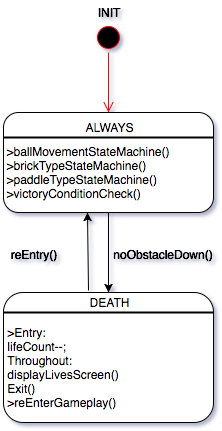
\includegraphics[width=4cm, height=8cm]{gameplayStateMachine}
\\ {\small Fig d: Gameplay State Machine}
\end{center}
\begin{lstlisting}[basicstyle = \small, language = C]
void displayOutput(void)
{
    while(1)
    {
        /*  Semaphore_pend(*sem, wait/timeout) 
         *  decrements the semaphore by 1.
         *  Until semaphore value is zero task is 
         *  blocked.
         *
         */
        Semaphore_pend(displayOutputSem, BIOS_WAIT_FOREVER);

        // Once Semaphore is posted, Switching State Machine 
        // uses different game states to dictate output 
        // behaviour
        switch(mode){
        case MENU:
            // In the Menu state
            switch(menuMode){
            case ENTRY:
                // Upon Entry, performed Once
                cursorPos = ONE;
                glcd_write(menuScreen);
                mode = MENU;
                displaySmallText("PLAY", 3, 6);
                displaySmallText("INSTRUCTIONS", 5, 2);
                displaySmallText("SETTINGS", 7, 4);
                menuMode = THROUGHOUT; 
                // Switch to THROUGHOUT internal state
                startBeep();
                break;
            case THROUGHOUT:
                // Performed throughout
                cursorDisplay(); 
                // Cursor position is switched accordingly as 
                // per cursor states
                break;
            }
            break;
            case INSTRUCTIONS:
                // In the Instructions State
                displaySmallText("USE THUMB STICK 
                TO MOVE PADDLE", 0, 0);
                displaySmallText("YOU HAVE THREE  LIVES", 3, 0);
                displaySmallText("CLEAR ALL BRICKS", 6, 0);
                displaySmallText("ALL THE BEST!", 7, 0);
                break;
            case SETTINGS:
                // In the Settings State
                displaySmallText("DIFFICULTY", 3, 2);
                // Based on user input (in readInput() task) 
                // display different difficulty modes as selected, 
                // on screen.
                switch(difficulty){
                case EASY:
                    displaySmallText("EASY  ", 4, 9);
                    break;
                case MEDIUM:
                    displaySmallText("HARD", 4, 9);
                    break;
                case HARD:
                    displaySmallText("INSANE", 4, 9);
                    break;
                }
                displaySmallText("BALL SPEED", 5, 2);
                // Based on user input (in readInput() 
                // task) display different ball speeds 
                // as selected, on screen.
                switch(ballSpeed){
                case SLOW:
                    displaySmallText("SLOW  ", 6, 9);
                    break;
                case FAST:
                    displaySmallText("FAST  ", 6, 9);
                    break;
                case FASTER:
                    displaySmallText("EXTREME", 6, 9);
                    break;
                }
                // Display cursor always
                cursorDisplay();
                break;
                case GAMEPLAY:
                    //In Gameplay State
                    switch(gameplayMode){
                    case ENTER:
                        // Performed once upon Entry
                        lifeCountTemp = lifeCount; 
                        // Maintain Temporary Life Count
                        score_str[0] = '0';
                        score_str[1] = '0';
                        score_str[2] = '0';
                        paddleXPos = 64;
                        paddleXPrev = paddleXPos; 
                        //Initial Paddle's previous 
                        // position is equal to its 
                        // current position
                        gameplayChange =NORMAL;
                        // Paddle size
                        // Based on difficulty, display 
                        appropriate number of lives screen
                        switch(difficulty){
                        case EASY:
                            screenFlash(threeLivesScreen);
                            break;
                        case MEDIUM:
                            screenFlash(twoLivesScreen);
                            break;
                        case HARD:
                            screenFlash(oneLifeScreen);
                            break;
                        }
                        // Set up Bricks Screen
                        gameScreen();
                        // Initialize ball variables
                        ballXPos = 7;
                        ballXPrev = 7;
                        ballYPos = 7;
                        ballYPrev = 7;
                        // Switch to ALWAYS internal state
                        gameplayMode = ALWAYS;
                        break;
                        case DEATH:
                            // Switch ON vibration motor 
                            // on DEATH
                            motorON();
                            // Performed upon Death
                            lifeCountTemp--; 
                            // Decrease number of lives
                            if(lifeCountTemp == 2)
                            {
                                // Re enter game after 
                                // displaying remaining 
                                // number of lives
                                screenFlash(twoLivesScreen);
                                gameplayMode = REENTER;
                            }
                            else if(lifeCountTemp == 1)
                            {
                                // Re enter game after 
                                // displaying remaining 
                                // number of lives
                                screenFlash(oneLifeScreen);
                                gameplayMode = REENTER;
                            }
                            else if(lifeCountTemp == 0)
                                mode = GAMEOVER;
                                // Switch to GAMEOVER 
                                // mode when player runs 
                                // out of lives
                            break;
                        case REENTER:
                            // Performed upon Re entry 
                            // after death. Re display 
                            // blocks remaining
                            gameScreenRefresh(); 
                            // Reset Ball Variables
                            ballXPos = 7;
                            ballXPrev = 7;
                            ballYPos = 7;
                            ballYPrev = 7;
                            // Set Ball direction
                            motorOFF(); 
                            // Switch OFF vibration motor
                            direction = INIT;
                            gameplayMode = ALWAYS; 
                            // Switch to ALWAYS internal 
                            // state
                            break;
                        case ALWAYS:
                            // Performed throughout
                            ballMovement();
                            // Check for victory condition 
                            satisfaction
                            if(victoryCheck == 1)
                                mode = VICTORY;
                            // Maintain LEDs in OFF state
                            ledOFF(1);
                            ledOFF(2);
                            ledOFF(3);
                            ledOFF(4);
                            break;
                    }
                    break;
                    case VICTORY:
                        // Performed when Victory condition is 
                        // satisfied
                        motorOFF();
                        victoryAnimationDisplay(); 
                        // Display a firework themed victory
                        animation
                        play_GOT(); 
                        // Play Game of Thrones Theme music 
                        // from Tones Library
                        glcd_write(creditsScreen); 
                        // Display Credits
                        millis(5000);
                        mode = MENU; // Return to Menu
                        menuMode = ENTRY;
                        break;
                    case GAMEOVER:
                        motorOFF();
                        direction = INIT; 
                        // Set Ball Direction
                        glcd_write(gameOverScreen); 
                        // Display Game Over Screen
                        displaySmallText(score_str, 5, 9); 
                        // Display Score
                        gameOverMusic(); 
                        // Play a short game over music from 
                        // the Tones Library
                        millis(2000);
                        glcd_write(creditsScreen); 
                        // Display Credits
                        millis(5000);
                        scoreInt = 0;
                        menuMode = ENTRY; // Return to Menuu
                        mode = MENU;
                        break;
        }
    }
}
  \end{lstlisting}
  
\texttt{main()}: \\ This function serves to initialize and start the BIOS. The BIOS handles program execution. Now, the \texttt{main()} function is defined as follows:
      \begin{lstlisting}[basicstyle = \small, language = C]
int main(void) {

    latency = 5;

    // Initialization of peripherals 
    // using functions in Console Directory
    _init_();
    glcd_init();
    glcd_clearDisplay();
    srand(time(NULL)); 
    // For Randomization of Blocks

    glcd_write(titleScreen); 
    // Display Cutscene
    play_MarioBros(); 
    // Play Mario Brothers Theme
    using Tones Library

    BIOS_start(); // Start BIOS

    return(0);
}
  \end{lstlisting}
\qquad The \texttt{Timer2\_ISR()} is defined, which is used to count to 10 seconds for the SPECIAL mode of the paddle when it hits BLOCK\_MAGIC2. Started on hit, and turned off on countdown.\\ \\
      \begin{lstlisting}[basicstyle = \small, language = C]
void Timer1_ISR(void)
{
    ROM_TimerIntClear(TIMER1_BASE, TIMER_TIMA_TIMEOUT);
    specialTimeCount++;
    if(specialTimeCount > 10000)
    {
        specialTimeCount = 0;
        gameplayChange = NORMAL;
        glcd_clearRow(7); 
        // Clear residual larger paddle 
        // (will remain displayed otherwise)
        specialExitBeep();
        // Disable Timer
        ROM_TimerDisable(TIMER1_BASE, TIMER_A);
        ROM_IntDisable(INT_TIMER1A);
        ROM_TimerIntDisable(TIMER1_BASE, TIMER_TIMA_TIMEOUT);
    }
}
  \end{lstlisting}
\qquad Finally, the \texttt{Timer2\_ISR()} is defined, which implements the task scheduling as shown: \\ \\
      \begin{lstlisting}[basicstyle = \small, language = C]
void Timer2_ISR(void)
{
    // Clear Interrupt
    ROM_TimerIntClear(TIMER2_BASE, TIMER_TIMA_TIMEOUT);
    tickCount++;
    switch(tickCount){
    case 10:
        Semaphore_post(displayOutputSem); 
        // Post Output Display Semaphore
        break;
    case 40:
        Semaphore_post(readInputSem); 
        // Post Input Read Semaphore
        tickCount=0;
        break;
    }
}
  \end{lstlisting}
This is the complete code for the Breakout Game, with a complete statechart implementation.
\end{document}
